\chapter{Motion Planning with Latent Human Intentions}\label{chap:hri}

Robots that are designed to assist humans almost inevitably have to operate in
a shared environment. \ac{hri} requires autonomous agents to navigate
safely in domains that typically do not feature safety barriers to physically
separate them from humans. Therefore, robots must ensure human safety through
careful planning and robust behaviors. At the same time, trajectories of humans
are hard to predict as they follow complex behaviors whose dynamics are only
partially understood.\todo{cite} For this reason, research in the past has
moved from simple rule-based and deterministic models \todo{social forces etc.}
towards data driven probabilistic predictions that approximate the future as
a distribution over trajectories \todo{cite: social lstm, and learning to
predict trajectories}.

\todo[inline]{Explain the notion of latent, internal state}

Incorporating stochasticity in the prediction pipeline allows the planner to
model uncertainty over both, high-level intentions (e.g. \emph{where} does the
human want to go), and low-level motion behavior (e.g. \emph{how} does the
human want to go there). Planning strategies that take this uncertainty into
account promise to provide robustified and potentially more efficient policies
for navigation around humans. While the properties gained from this kind of
planning are desirable for many \ac{hri} problems, reasoning over distributions
of possible futures may pose a challenging \ac{pomdp}. Therefore, a lot of
research has focused on recovering some of these properties by proposing domain
specific simplifications for these applications \cite{fern2007decision,
sadigh2016information, javdani2018shared, fisac2018probabilistically}.

On the other hand, recent research in this field suggests that through
increased performance of modern solvers, \ac{pomdp} approaches for motion
planning problems with \ac{hri} are becoming increasingly practical and that
this kind of reasoning can help to generate robustified and more efficient
behaviors for this domain. \cite{bai2015intention} use the \ac{despot} to
control the speed of an autonomous golf cart for navigation in a crowd. They
show that by reasoning over future observations the system is able to maneuver
more safely while reaching the goal faster and increasing passenger comfort
through smoother trajectories than the proposed greedy baseline.
\cite{sunberg2017value} examine the value of inferring the internal state of
traffic participants for autonomous freeway driving. The results presented in
their work show that the problem allows for a significant increase in
performance when the agent is omniscient to the individual internal state of
other vehicles compared to planning with a static \emph{normal} behavior for
all traffic participants. They demonstrate that inference of the latent
behavior parameters in combination with \ac{pomdp} planning allows to greatly
reduce the gap to the omniscient upper bound.

While a lot of work in motion planning under uncertainty has focus on either
\emph{problem specific simplifications} on the one hand or \emph{full
\ac{pomdp} solutions} on the other, few results exist on the direct comparison
of the two. In this chapter we consider a case of motion planning in the
presence of humans for which an elaborate domain specific strategy has been
proposed in \cite{fisac2018probabilistically}. This strategy simplifies the
planning problem by neglecting future observations. Instead, human prediction
are performed on expectation from the current belief, providing series of
probability maps for future human lotions. The authors propose a method that
allows planning with these probabilistic predictions by means of conventional
motion planning algorithms. We implement this strategy in the \pomdpsjl
framework to compare it's performance with behaviors generated by
\ac{pomcpow}.

We begin by stating the details of the motion planning problem in
\cref{sec:hri-problem-statement}. \cref{sec:hri-pomdp-formalization} then
formalizes this problem as a \ac{pomdp}. \cref{sec:hri-solutions} briefly
presents the domain specific approximate planner proposed in
\cite{fisac2018probabilistically}, as well as the \ac{pomcpow} solver adapted
for this problem. Finally, we evaluate the performance of both policies and
discuss the results in \cref{sec:hri-evaluation}.

\section{Problem Statement}\label{sec:hri-problem-statement}

In this chapter we study a motion planning problem for a robot in a shared
environment with a human actor. The assumptions made for this planning problem
aim to closely match the setup described in \cite{fisac2018probabilistically}.

\todo[inline]{add screenshot of simulator}

\paragraph{High Level Problem}

Consider a human and a robot navigating in a common environment. As a running
example, this problem may be envisioned as an indoor navigation problem. In
this problem, the robot aims to efficiently reach a preset goal location
inside the room while trying to avoid collisions with the human. At the same
time, the human does not pay attention to the robot. That is, the decisions of
the human actor do not depend on the location of the robot. Furthermore, the
human has time-varying intentions that are not known by the robot. At every
time step the human aims to reach a certain goal inside the room. Once arrived
at this goal, the human may either stay at this goal or proceed to another goal
location. Furthermore, the human has a small likelihood of changing the
intended walk target mid way. The robot has a model for some of the locations
humans might want to go to. However, the planner neither knows the exact path
the human will take, nor is it's model of human goals complete. That is, the
person might aim to reach an unmodeled goal location. At every time step the
robot receives a perfect observation of the current position of both itself and
the human. The robot ultimately needs to plan and execute a trajectory to
a goal state according to some notion of efficiency, while avoiding collisions
with the human.

\paragraph{Human Behavior Model}

This problem poses a challenging planning problem as it requires the agent to
carefully reason about the intentions of the human in order to avoid collisions
while trying to reach it's own goal. Furthermore, in order to be robust against
cases in which the person tries to approach an unmodeled goal, the agent needs
to make safe fall-back predictions when the human behaves unexpectedly. At the
same time, planning with the worst case assumption by trying to avoid the
humans forward reachable set is too conservative.

In this problem setting, the robot is assumed to have access to suitable human
reward function. In practice such reward model can be learned offline from
prior human demonstrations, e.g. using inverse reinforcement
learning\todo{cite?}. By means of a noisy-rationality model used in cognitive
science \cite{baker2007goal}, the planner can make probabilistic predictions
of human actions given the state,

\begin{equation}\label{eq:boltzmann}
  P\left(a^t_\text{H} | s^t_\text{H}; \beta, \theta \right) \propto e^{\beta Q_\text{H}\left(s^t_\text{H}, a^t_\text{H}; \theta\right)}.
\end{equation}

Here, $a^t_\text{H}$ is the human action taken at time $t$; $s^t_\text{H}$ is
the state of the human at this time; $Q_\text{H}(s_\text{H}, a_\text{H}; \theta)$ is the
state-action value function of the human, with $\theta$ being the parameters of the
$Q$-value encoding latent human intentions (e.g. the goal location); $\beta$ is
the so called \emph{rationality coefficient}.\\
This model encodes the assumption that humans are more likely to select actions that
provide a higher $Q$-value. The rationality constant, $\beta$, determines the
degree to which the robot expects the human to align with the provided reward
model. For $\beta = 0$ the model in \cref{eq:boltzmann} degenerates to
a uniform distribution over all actions. For $\beta \to \infty$ the human acts
perfectly rational with respect to the utility model,
$Q_\text{H}$.

Here, we treat both $\theta$ and $\beta$ as latent parameters. That is, the
agent needs to reason over the parameters of the human reward model (e.g. it's
current goal) as well as the accuracy of this model.

\section{POMDP Formalization}\label{sec:hri-pomdp-formalization}

The problem is formalized as a \ac{pomdp} from the robot perspective. It is
characterized by the following properties introduced in \cref{sec:pomdp}:

\begin{description}
  \item[State Space $\sspace$.] The state of the environment is defined as the
  joint state of the human and the robot. For clarity, we introduce the
  subscripts $H$ and $R$ to denote the affiliation of a subset of the state to
  the human or the robot, respectively. Furthermore, we differentiate between
  \emph{external states} (i.e. states that encode physical properties of the
  environment) and \emph{internal states} (i.e. states that determine the
  behavior dynamics of an agent), denoted with subscript $E$ and $I$,
  respectively. Using this notation, a state state variable $s$ is composed as:
  \begin{equation}
    s = [s_\text{E,R}, s_\text{E,H}, s_\text{I,H}]^T
  \end{equation}
  It is important to note that, in order to make $s$ Markovian, we need to
  incorporate the internal state of the human. That is, in contrast to a game theoretic
  approach, humans are not explicitly modeled as players taking actions but
  rather in terms of dynamics of the environment. In the model of the robot, the
  human internal state consists of the reward model parameters, $\theta$, and
  the model confidence, $\beta$. The external state of each actor is defined
  by it's current position.

  Using this definition of the state, $\sspace$ is the set of all possible
  combinations of positions the human and the robot and the human internal state.
  \item[Action Space $\aspace$.] An action in this problem refers
  \emph{exclusively} to the robot action. At every time step the robot can select
  one of the following six actions:
  \emph{"north", "east", "south", "west", "to goal", and "stay put"}. The keep
  the robot at it's current position. All other actions ill move the agent with
  constant velocity in the corresponding direction. Here, \emph{to goal} is
  a state dependent action, that is directed straight at the robot's goal
  location. The set of these six actions constitutes the action space, $\aspace$.
  \item[Transition Model $\tdist$.] The dynamics of the robot and the human are
    decoupled. Therefore, we can compose the joint state transition from the
    dynamics of each actor. The transition of the robot, $s_\text{R}$ to
    $s_\text{R}'$, depends on the action as described above. The transition of
    the human obeys \cref{eq:boltzmann}. In our model, the human has
    a discretized action space that allows it to stay put or move in one out of
    eight preset directions (i.e. \emph{north}, \emph{north-east},
    \emph{east}...). Hence, at every time step the human action is generated by
    sampling from the generalized Bernoulli obtained from \cref{eq:boltzmann}
    and the human is moved in the corresponding direction. Additionally, the
    transitions of both actors are corrupted by Gaussian process noise. A terminal
    state is reached if either the robot collides with the human or it reaches the goal.
  \item[Reward Function $\reward: \sspace \times \aspace \times
    \sspace \to \reals$.] The reward model of the robot is defined as:
    \begin{equation}
      \reward(s, a, s') = r_\text{time} + \chrond_\text{collision}(s') r_\text{collision} + \chrond_\text{close}(s') r_\text{close}.
    \end{equation}
    The reward model is parametrized by the following quantities:
    $r_\text{time}$ is a living penalty encouraging the robot to minimize the
    time until the goal is reached; $r_\text{collision}$ is a penalty for
    collision with the human or the walls of the room; $r_\text{close}$ is the
    penalty obtained when entering the one-step forward reachable set of the human.\\
  \item[Discount Factor $\gamma$.] Rewards are discounted with $\gamma = 0.99$.
  \item[Observation Space $\ospace$.] At every time step the robot receives an
    exact measurement of the human and itself. That is, the robot gets to observe
    the external state, $s_\text{E}$ of both actors. As a result, $\ospace$ is
    strict subset of the state space.
  \item[Observation Model $\odist$.] Since the position sensor is exact, the observation
    model is a Dirac delta function, evaluating non-zero for a state, $s$, if and
    only if the external state component matches the observation, $o$.
\end{description}

It must be noted that, in order to match the problem statement provided in
\cref{sec:hri-problem-statement}, we consider two slightly different versions
of this \ac{pomdp}. One version is used to represent the dynamics of the simulated
environment, the other is used as a planning model for the robot. This clear
distinction is necessary to encode the modelling assumption that the robot does not
know about all human goals. That is, the robot does not have access to the true
behavior model of the human.

By inspection of the problem formalized above it becomes apparent that the
assumptions made in \cite{fisac2018probabilistically} poses a \ac{momdp} --
a special case of the more general \ac{pomdp}. That is, we can factor the state
into a fully observed part ($s_\text{E}$, the external state) and a partially
observed part ($s_\text{I}$).

% \todo[inline]{Point to the corresponding implementations of these things. This
% is the best way of communicating further details.}

\section{Solution Strategies}\label{sec:hri-solutions}

We solve the \ac{pomdp} described in \cref{sec:hri-pomdp-formalization} using
two different strategies. First, \cref{sec:hri-baseline} presents
\ac{psrp}, a method proposed in \cite{fisac2018probabilistically} that exploits
the special structure of the problem to reduce the computational effort of
solving the full \ac{pomdp}. Thereafter, \cref{sec:hri-planners} presents an
adaptation of \ac{pomcpow} for this problem.

% \todo[inline]{Maybe point to the
% fact that one could also use \ac{despot}, but that we found \ac{pomcpow} to
% work better (data of Andreea) and that the point of this section is rather to
% compare POMDP vs non-pomdp approaches rather than solver internal benchmark.}

\subsection{Probabilistically Safe Robot Planning}\label{sec:hri-baseline}

\acf{psrp} is a method for motion planning with probabilistic predictions.
While an exhaustive discussion of the details of this method is beyond the
scope of this work, we aim to provide insight into the general idea of this
method as a basis for further discussion. For additional information the reader
may refer to the original paper \cite{fisac2018probabilistically}.

\ac{psrp} is designed for a special class of \acp{pomdp} with the following
properties: The problem must be a \acp{momdp} in which the notion of
\emph{immediate safety} can be evaluated solely on fully observed states.
Furthermore, all such state components affecting immediate safety must be
either \emph{actuated} (i.e. directly controlled by the agent) or \emph{fully
decoupled} from the robot dynamics to allow for predictions independent of the
agent's decisions. Both requirements are satisfied for the problem studied in
this chapter: Immediate safety depends only on the position of the human and
the robot, both contained in the \emph{external} (fully observed) part of the
state; Predictions of the human state can be made independently of the robots
trajectory as she ignores the robot position in her decision making process.

The methods exploits these properties to significantly reduce the complexity of
policy search by essentially converting it to an equivalent non-probabilistic
formulation. The converted problem can then be solved using conventional
motion-planning techniques. On an abstract level the algorithmic procedure of
\ac{psrp} performs the following computations to select the next action:

\begin{description}
  \item[Inference / Belief Update] At every times step the robot receives an
    exact observation of the external state of the environment. These
    observations are used to maintain a belief over the latent parameters of
    the human model presented in \cref{eq:boltzmann}. These are the goal
    location of the human, $\theta$, and the model confidence, $\beta$. The
    exact update of the joint belief takes the form \begin{equation} b'(\theta,
    \beta) \propto P(s_\text{E,H} | s_\text{H}; \theta, \beta) b(\theta,
    \beta). \end{equation} Since the exact Bayesian update is computationally
    demanding, we perform Monte-Carlo integration to run the inference. Note
    that this is a subtle difference to the original implementation, where the
    authors decide the discretize the parameter and state space to obtain
    a tractable update rule.
  \item[Prediction] Using the belief provided by the inference, the agent
    computes a probabilistic prediction of the human position for $K$ future
    time steps. This is done by recursively propagating the particles belief
    through a generative model matching the statistics of \cref{eq:boltzmann}.
    Since the human is modeled to act noisily rational and additionally the
    particle belief represents a distribution over possible human behaviors,
		the prediction introduces uncertainty to the future trajectory of the
		human. That is, while at the current time step the exact position of the
 		human is known from the most recent observation, at future times the
	  robot only has a probabilistic estimate of the person's location.
    An example of such open-loop predictions of the human location is depicted
    in \cref{fig:psrp-prediction-example}. These predictions are used to
    synthesize a probabilistic obstacle map for the next $K$ time steps.
  \item[Planning] The agent uses the $K$ probabilistic obstacle maps obtained
    from the preceding step to compute the optimal sequence of actions for the
    next $K$ time steps. Since the action-space is finite, we use $A^\ast$ to
    solve this policy search problem. We use the negative reward model as
    a cost function to obtain the cost function for the graph search problem.
    Additionally, in line with the idea of \cite{fisac2018probabilistically} we
    prune search nodes for which the collision likelihood exceeds a preset
    threshold, $\varepsilon$.
\end{description}

The result of this computation is applied in the fashion of a $K$-step receding
horizon \ac{mpc}. That is, at every time step the robot only executes the first
action of the optimal action sequence computed above. At the next time step,
all steps are repeated closing the loop over the received observation.

\todo[inline]{@zach: should this feature additional implementation details
(e.g. KDTree for nearest neighbour search etc?)}

\begin{figure}[htpb]
  \centering
  \missingfigure{Example of probabilistic predictions}.
  \caption{Exemplary predictions of the human future location in \acf{psrp}.\todo[inline]{Refine caption once figure is finished.}}
  \label{fig:psrp-prediction-example}
\end{figure}

\subsection{POMCPOW}\label{sec:hri-planners}

The \ac{pomdp} formalization presented in \cref{sec:hri-pomdp-formalization}
allows to directly apply \ac{pomcpow} to the problem. To ensure a fair
comparison, the planner uses the same particle filter as proposed for \ac{psrp}
in \cref{sec:hri-baseline} for inference of the latent parameters of the human model.

Considering the insight obtained from the solver comparison discussed in
\cref{chap:localization-and-planning}, we choose to embed domain knowledge
through an analytic value estimate. Using the same kind of reasoning as
discussed in \cref{sec:lp-planners-pomcpow} we approximate the value at the
leaf of the policy tree using a relaxed version of the problem in which the
robot can move on a straight, collision-free line to it's goal location. By
means of this relaxation, the value estimate is given as the discounted sum of
living penalties over the reaming steps to the goal.

\section{Evaluation and Discussion}\label{sec:hri-evaluation}

We evaluate the performance of each strategy by running $5000$ simulations for
each policy. Again, each policy is simulated on the same set of random seeds to
reduce sampling variance. Additionally, in an effort to obtain a comparison
that focuses on safety critical situations, we only consider scenarios in which
a naive \emph{straight-to-goal} policy is not successful. We create these
scenarios by sampling initial conditions from uniform prior and reject all
samples for which the simulated naive policy allows the robot to reach it's goal.

In contrast to the experiments presented in
\cref{chap:localization-and-planning}, we don't explicitly set an upper bound
on the decision time per step for \ac{pomcpow} but fix the number of
\ac{mcts} iterations instead. We choose the number of iterations by evaluating the
performance of \ac{pomcpow} over a sequence of parameters and select the number
of iterations beyond which saturation is observed. Furthermore, for the
experiments discussed we are able to simulate all policies until a terminal
state is reached. Hence, we don't need to adjust the returns to account for
rewards beyond the simulated horizon. Additionally, we limit the planning horizon
for both solvers to ten steps to avoid any bias due to unbalanced prescience.

We begin by comparing the performance of each policy by examining the
cumulative discounted reward -- the metric whose maximization is the objective
of this optimization problem. \Cref{fig:hri_eval_value_sem} shows the mean and
\ac{sem} of the cumulative discounted reward for $5000$ experiments over both
policies. These results show that \ac{pomcpow} performs significantly better
than \ac{psrp}.

\begin{figure}[htpb]
  \centering
  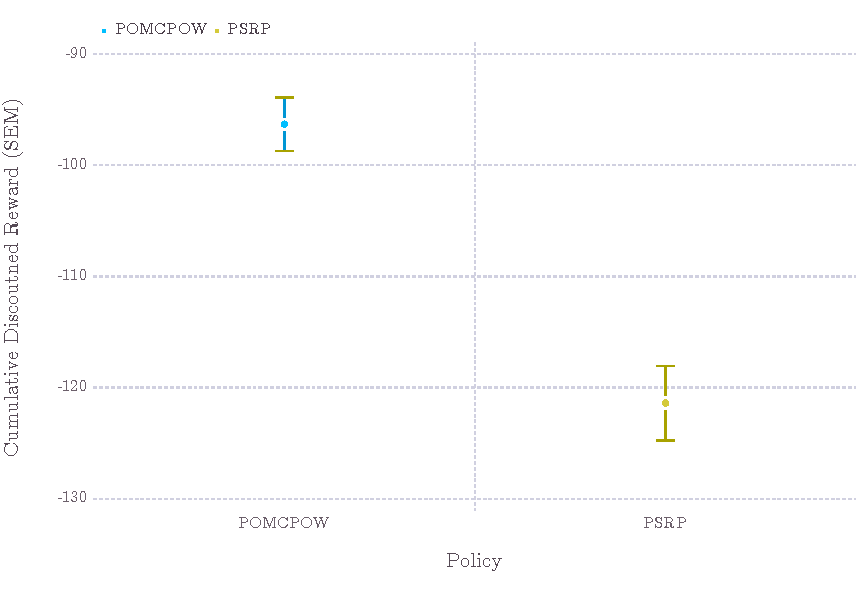
\includegraphics[scale=1]{hri_plots/hri_value_sem_plot.pdf}
  \caption{Mean and \acf{sem} of the cumulative discounted reward for
  \ac{pomcpow} (blue) and \ac{psrp} (yellow) as introduced in \cref{sec:hri-solutions}.}
  \label{fig:hri_eval_value_sem}
\end{figure}

Further insight is gained by evaluating the outcome statistics for each policy.
\Cref{fig:hri_outcome_histogram} depicts the frequencies of outcomes for each
policy. Since both policies reach a terminal state within the simulated horizon
for all sampled scenarios, here we only consider two classes of outcomes:
\emph{success}, the robot reached the goal location; and \emph{failure} the
robot collided with a wall or the human. The outcome statistics show that both
policies are able to successfully navigate the robot to it's goal location in
the vast majority of all scenarios. However, \ac{pomcpow} still performs
significantly better with respect to safety. In fact, the collision rate in the
sampled scenarios for \ac{pomcpow} ($3.40\%$) is only half has high as for
\ac{psrp} ($7.08\%$).
% \todo[inline]{Should I note the adversarial character of these examples: many scenarios are rejected}

\begin{figure}[H]
  \centering
  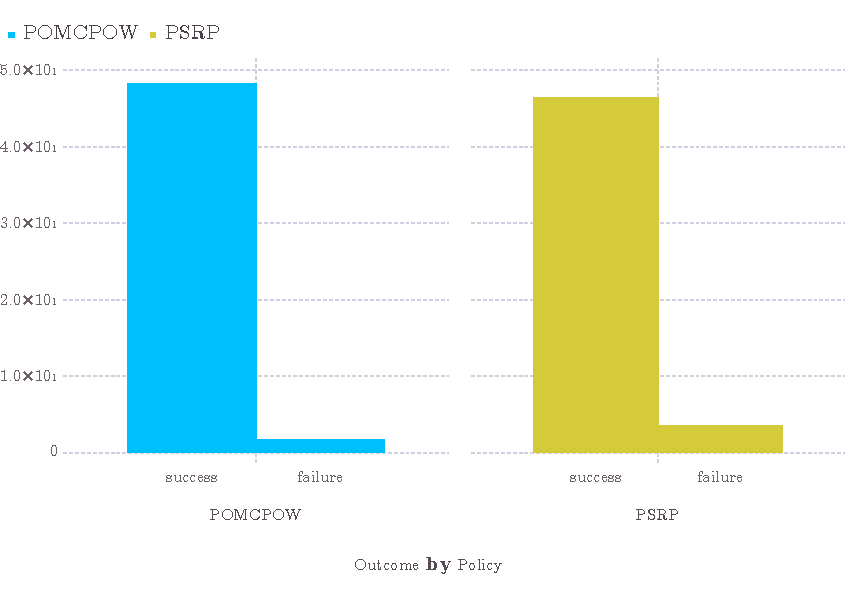
\includegraphics[scale=1]{hri_plots/hri_outcome_histogram_plot.pdf}
  \caption{Histogram of outcome frequencies grouped by policy. Outcome classes:
  \emph{success}, the robot reached the goal location; and \emph{failure} the
  robot collided with a wall or the human.}
  \label{fig:hri_outcome_histogram}
\end{figure}

While \ac{pomcpow} provides quantifiable better behaviors, this advantage comes
at the cost of higher computational effort. On average, decision making in
\ac{pomcpow} takes $\SI{0.279}{s}$ while for \ac{psrp} a decision is computed
within $\SI{0.042}{s}$.

A qualitative analysis of the behaviors generated by each solvers provides
further insight into the reasons for this gap in performance. We observe that
in many cases both solvers follow very similar strategies. When the human walks
towards one of the goal locations known by the robot, her decisions are well
explained by the behavior model used by the planner. In these cases, the model
confidence, $\beta$, increases and the planner is able to make confident
predictions of the future human position. Hence, for sufficiently high values
of $\beta$ the problem essentially approaches a deterministic planning problem.
Under these conditions \ac{psrp} performs equally well as \ac{pomcpow} since
optimal planning with probabilistic obstacles reliably finds suitable
trajectories to avoid collisions and reach the goal efficiently. In fact, in
the limit of $\beta \to \infty$ observation branching as employed by
\ac{pomcpow} is rendered obsolete.

Furthermore, in the problem discussed here the human does not react to the
robot. Therefore, observations whose statistics depend on latent variables are
independent of the robot action. As a result, in contrast to the application
domain discussed in \cref{chap:localization-and-planning} this problem does not
enable active information gathering. This property induced by the problem
structure further reduces the effect of observation branching.\\ However, there
still is a decisive difference between both strategies that causes the
performance gap observed above. In cases where the human appears to act
irrational the model confidence decreases and \cref{eq:boltzmann} essentially
becomes a uniform distribution. As as a result, the sequence of probabilistic
predictions used in \ac{psrp} features rapidly expanding uncertainty and the
planner has to avoid a large region of the state space. We observe that during
these maneuvers the agent often gets trapped in a corner of the room. When
using \ac{pomcpow} on the other hand, the agent is aware that it will get
further information to reduce the uncertainty in the future. Hence, the agent
is able to approach the human more confidently, enabling the robot to navigate
around the human in a less reactive manner.

In summary we can state that for the application example discussed in this
chapter the difference between the domain specific solver, \ac{psrp}, and the
generic \ac{pomdp} solver, \ac{pomcpow}, is less dramatic. Since by design the
problem does not allow for active information gathering, in many cases both
solvers generate similar behaviors. However, when faced with significant
uncertainty over the human intention, \ac{pomcpow} is still able to navigate
more safely, since observation branching allows to keep uncertainty over future
human positions bounded.

%  \begin{figure}[htpb]
%    \centering
%    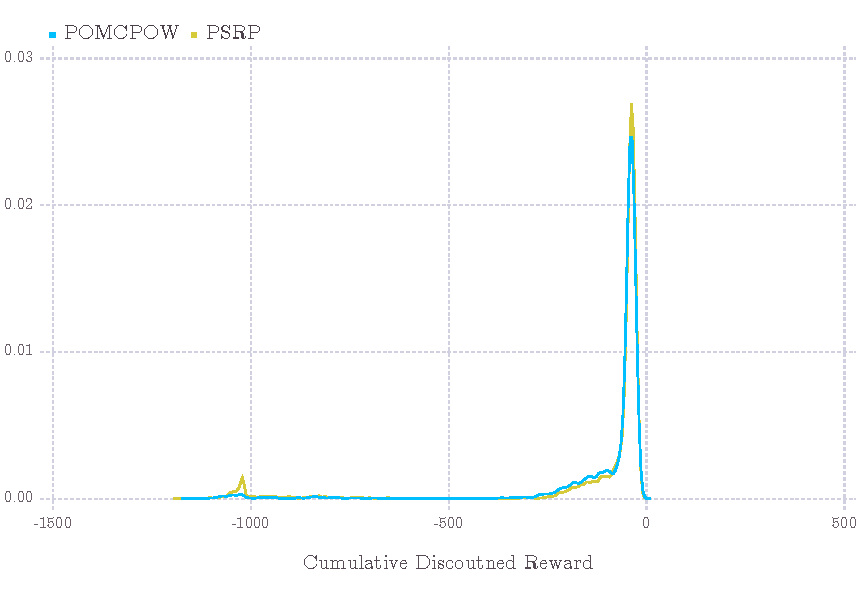
\includegraphics[scale=1]{hri_plots/hri_value_density_plot.pdf}
%    \caption{TODO}
%    \label{fig:hri_eval_value_density}
%  \end{figure}
%  
%  \begin{figure}[htpb]
%    \centering
%    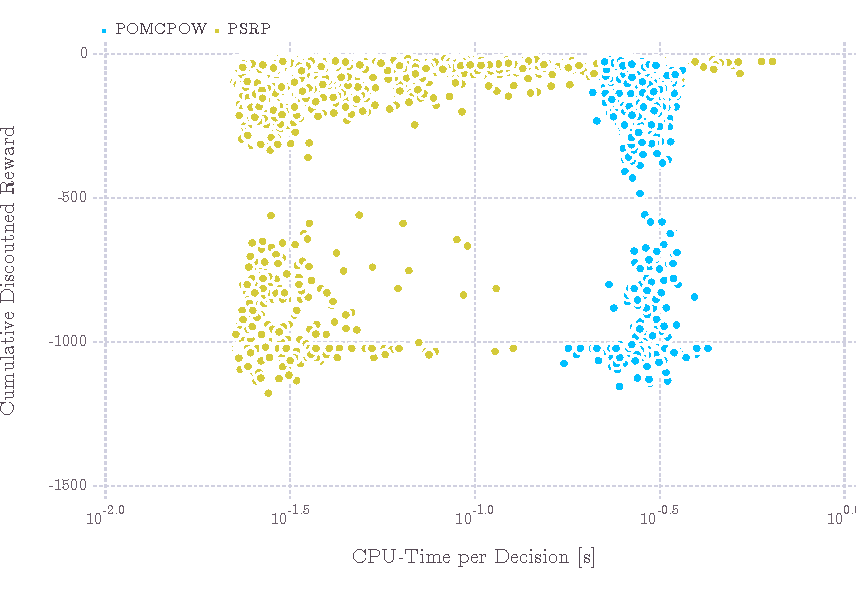
\includegraphics[scale=1]{hri_plots/hri_value_compute_scatter_plot.pdf}
%    \caption{TODO}
%    \label{fig:hri_eval_value_compute_scatter}
%  \end{figure}
%  
%  \begin{figure}[htpb]
%    \centering
%    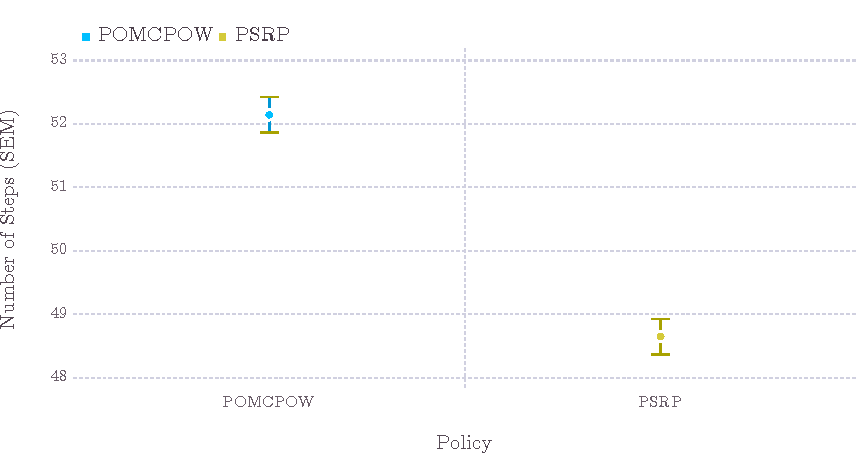
\includegraphics[scale=1]{hri_plots/hri_nstep_sem_plot.pdf}
%    \caption{TODO}
%    \label{fig:hri_eval_nstep_sem}
%  \end{figure}
%  
%  \begin{figure}[htpb]
%    \centering
%    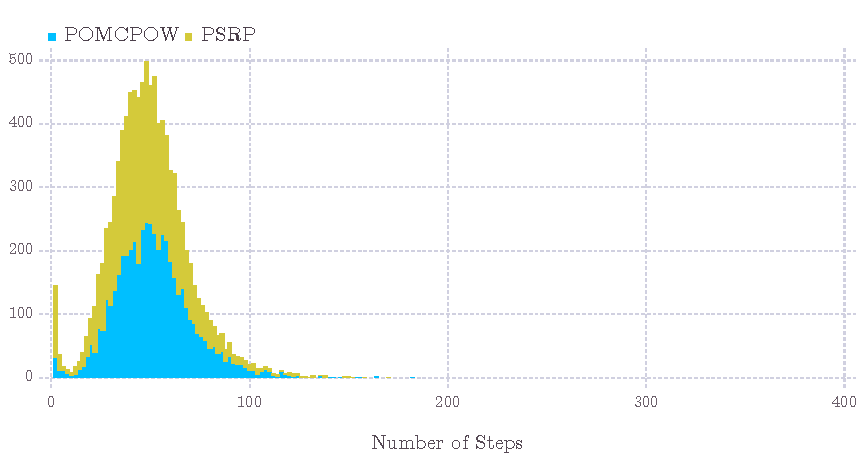
\includegraphics[scale=1]{hri_plots/hri_nstep_density_plot.pdf}
%    \caption{TODO}
%    \label{fig:hri_eval_nstep_density}
%  \end{figure}
%  
%  \begin{figure}[htpb]
%    \centering
%    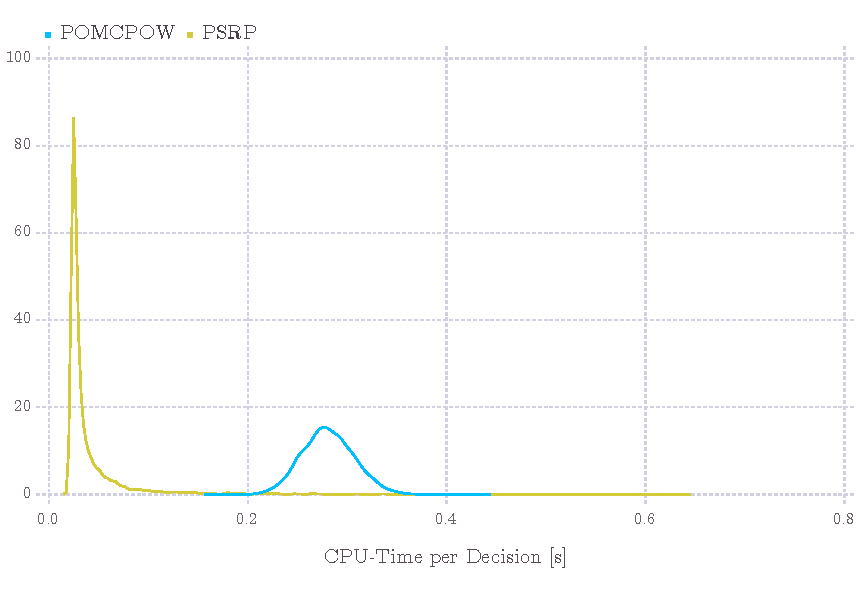
\includegraphics[scale=1]{hri_plots/hri_compute_density_plot.pdf}
%    \caption{TODO}
%    \label{fig:hri_eval_compute_density}
%  \end{figure}
